% ANEXO------------------------------------------------------------------------

\begin{anexosenv}
\partanexos

% Primeiro anexo---------------------------------------------------------------
\chapter{Nova Resolução de ACC dos Cursos da FACEEL}     % edite para alterar o título deste anexo
\label{anexo:novaResolucaoDeACC}

% Lembre-se que a diferença entre apêndice e anexo diz respeito à autoria do texto e/ou material ali colocado.

% Caso o material ou texto suplementar ou complementar seja de sua autoria, então ele deverá ser colocado como um apêndice. Porém, caso a autoria seja de terceiros, então o material ou texto deverá ser colocado como anexo.

% Caso seja conveniente, podem ser criados outros anexos para o seu trabalho acadêmico. Basta recortar e colar este trecho neste mesmo documento. Lembre-se de alterar o "label"{} do anexo.

% Organize seus anexos de modo a que, em cada um deles, haja um único tipo de conteúdo. Isso facilita a leitura e compreensão para o leitor do trabalho. É para ele que você escreve.

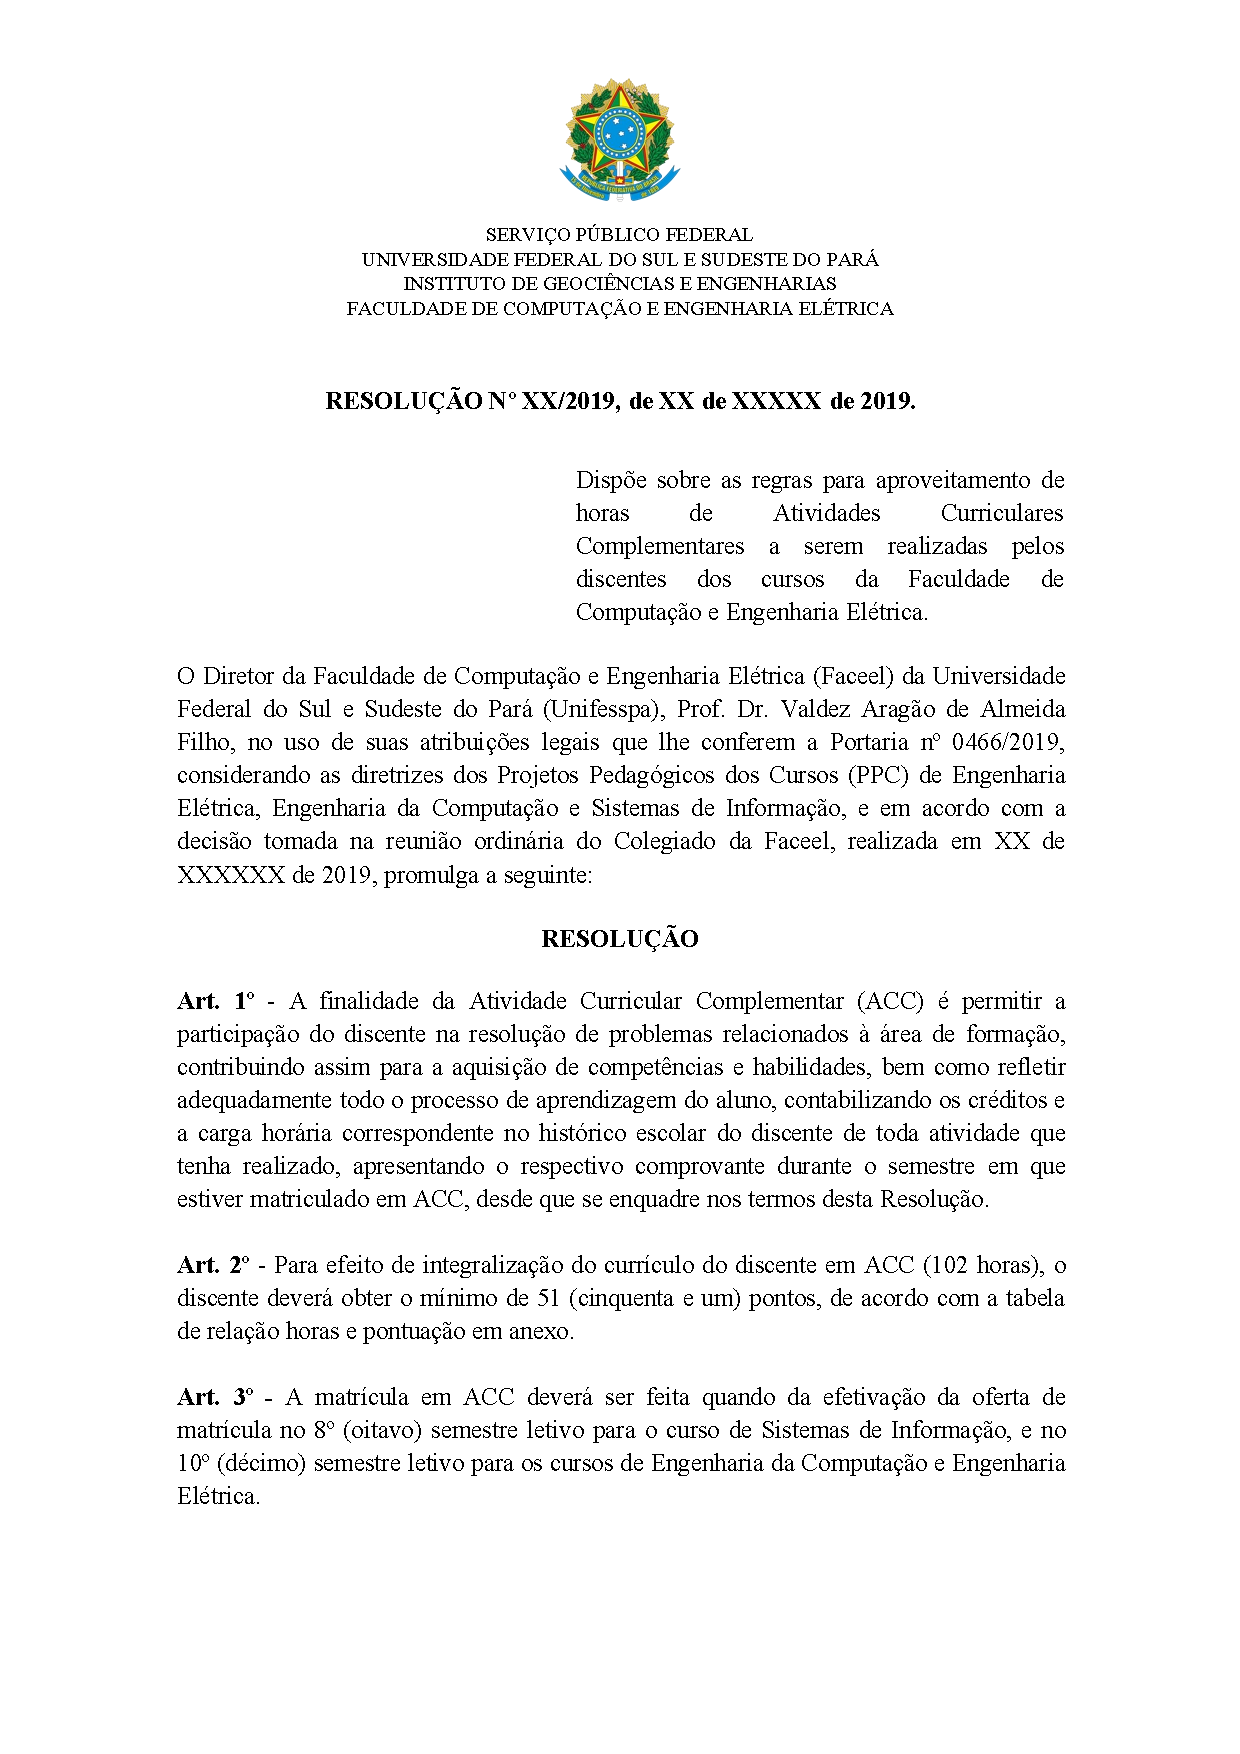
\includepdf[pages=-]{dados/anexos/regulamento_acc.pdf}

% Novo anexo-------------------------------------------------------------------
% \chapter{Nome do outro anexo}
% \label{chap:anexoB}

% conteúdo do outro anexo

\end{anexosenv}
